% Options for packages loaded elsewhere
\PassOptionsToPackage{unicode}{hyperref}
\PassOptionsToPackage{hyphens}{url}
%


\PassOptionsToPackage{table}{xcolor}

\documentclass[
  10pt,
  letterpaper,
]{article}

\usepackage{amsmath,amssymb}
\usepackage{lmodern}
\usepackage{iftex}
\ifPDFTeX
  \usepackage[T1]{fontenc}
  \usepackage[utf8]{inputenc}
  \usepackage{textcomp} % provide euro and other symbols
\else % if luatex or xetex
  \usepackage{unicode-math}
  \defaultfontfeatures{Scale=MatchLowercase}
  \defaultfontfeatures[\rmfamily]{Ligatures=TeX,Scale=1}
\fi
% Use upquote if available, for straight quotes in verbatim environments
\IfFileExists{upquote.sty}{\usepackage{upquote}}{}
\IfFileExists{microtype.sty}{% use microtype if available
  \usepackage[]{microtype}
  \UseMicrotypeSet[protrusion]{basicmath} % disable protrusion for tt fonts
}{}
\makeatletter
\@ifundefined{KOMAClassName}{% if non-KOMA class
  \IfFileExists{parskip.sty}{%
    \usepackage{parskip}
  }{% else
    \setlength{\parindent}{0pt}
    \setlength{\parskip}{6pt plus 2pt minus 1pt}}
}{% if KOMA class
  \KOMAoptions{parskip=half}}
\makeatother
\usepackage{xcolor}
\usepackage[top=0.85in,left=2.75in,footskip=0.75in]{geometry}
\setlength{\emergencystretch}{3em} % prevent overfull lines
\setcounter{secnumdepth}{-\maxdimen} % remove section numbering


\providecommand{\tightlist}{%
  \setlength{\itemsep}{0pt}\setlength{\parskip}{0pt}}\usepackage{longtable,booktabs,array}
\usepackage{calc} % for calculating minipage widths
% Correct order of tables after \paragraph or \subparagraph
\usepackage{etoolbox}
\makeatletter
\patchcmd\longtable{\par}{\if@noskipsec\mbox{}\fi\par}{}{}
\makeatother
% Allow footnotes in longtable head/foot
\IfFileExists{footnotehyper.sty}{\usepackage{footnotehyper}}{\usepackage{footnote}}
\makesavenoteenv{longtable}
\usepackage{graphicx}
\makeatletter
\def\maxwidth{\ifdim\Gin@nat@width>\linewidth\linewidth\else\Gin@nat@width\fi}
\def\maxheight{\ifdim\Gin@nat@height>\textheight\textheight\else\Gin@nat@height\fi}
\makeatother
% Scale images if necessary, so that they will not overflow the page
% margins by default, and it is still possible to overwrite the defaults
% using explicit options in \includegraphics[width, height, ...]{}
\setkeys{Gin}{width=\maxwidth,height=\maxheight,keepaspectratio}
% Set default figure placement to htbp
\makeatletter
\def\fps@figure{htbp}
\makeatother

% Use adjustwidth environment to exceed column width (see example table in text)
\usepackage{changepage}

% marvosym package for additional characters
\usepackage{marvosym}

% cite package, to clean up citations in the main text. Do not remove.
% Using natbib instead
% \usepackage{cite}

% Use nameref to cite supporting information files (see Supporting Information section for more info)
\usepackage{nameref,hyperref}

% line numbers
\usepackage[right]{lineno}

% ligatures disabled
\usepackage{microtype}
\DisableLigatures[f]{encoding = *, family = * }

% create "+" rule type for thick vertical lines
\newcolumntype{+}{!{\vrule width 2pt}}

% create \thickcline for thick horizontal lines of variable length
\newlength\savedwidth
\newcommand\thickcline[1]{%
  \noalign{\global\savedwidth\arrayrulewidth\global\arrayrulewidth 2pt}%
  \cline{#1}%
  \noalign{\vskip\arrayrulewidth}%
  \noalign{\global\arrayrulewidth\savedwidth}%
}

% \thickhline command for thick horizontal lines that span the table
\newcommand\thickhline{\noalign{\global\savedwidth\arrayrulewidth\global\arrayrulewidth 2pt}%
\hline
\noalign{\global\arrayrulewidth\savedwidth}}

% Text layout
\raggedright
\setlength{\parindent}{0.5cm}
\textwidth 5.25in 
\textheight 8.75in

% Bold the 'Figure #' in the caption and separate it from the title/caption with a period
% Captions will be left justified
\usepackage[aboveskip=1pt,labelfont=bf,labelsep=period,justification=raggedright,singlelinecheck=off]{caption}
\renewcommand{\figurename}{Fig}

% Remove brackets from numbering in List of References
\makeatletter
\renewcommand{\@biblabel}[1]{\quad#1.}
\makeatother

% Header and Footer with logo
\usepackage{lastpage,fancyhdr}
\usepackage{epstopdf}
%\pagestyle{myheadings}
\pagestyle{fancy}
\fancyhf{}
%\setlength{\headheight}{27.023pt}
%\lhead{\includegraphics[width=2.0in]{PLOS-submission.eps}}
\rfoot{\thepage/\pageref{LastPage}}
\renewcommand{\headrulewidth}{0pt}
\renewcommand{\footrule}{\hrule height 2pt \vspace{2mm}}
\fancyheadoffset[L]{2.25in}
\fancyfootoffset[L]{2.25in}
\lfoot{\today}
\makeatletter
\makeatother
\makeatletter
\makeatother
\makeatletter
\@ifpackageloaded{caption}{}{\usepackage{caption}}
\AtBeginDocument{%
\ifdefined\contentsname
  \renewcommand*\contentsname{Table of contents}
\else
  \newcommand\contentsname{Table of contents}
\fi
\ifdefined\listfigurename
  \renewcommand*\listfigurename{List of Figures}
\else
  \newcommand\listfigurename{List of Figures}
\fi
\ifdefined\listtablename
  \renewcommand*\listtablename{List of Tables}
\else
  \newcommand\listtablename{List of Tables}
\fi
\ifdefined\figurename
  \renewcommand*\figurename{Figure}
\else
  \newcommand\figurename{Figure}
\fi
\ifdefined\tablename
  \renewcommand*\tablename{Table}
\else
  \newcommand\tablename{Table}
\fi
}
\@ifpackageloaded{float}{}{\usepackage{float}}
\floatstyle{ruled}
\@ifundefined{c@chapter}{\newfloat{codelisting}{h}{lop}}{\newfloat{codelisting}{h}{lop}[chapter]}
\floatname{codelisting}{Listing}
\newcommand*\listoflistings{\listof{codelisting}{List of Listings}}
\makeatother
\makeatletter
\@ifpackageloaded{caption}{}{\usepackage{caption}}
\@ifpackageloaded{subcaption}{}{\usepackage{subcaption}}
\makeatother
\makeatletter
\makeatother
\ifLuaTeX
  \usepackage{selnolig}  % disable illegal ligatures
\fi
\usepackage[numbers,square,comma]{natbib}
\bibliographystyle{plos2015}
\IfFileExists{bookmark.sty}{\usepackage{bookmark}}{\usepackage{hyperref}}
\IfFileExists{xurl.sty}{\usepackage{xurl}}{} % add URL line breaks if available
\urlstyle{same} % disable monospaced font for URLs
\hypersetup{
  pdftitle={Exploring Zstandard user-provided dictionary compression for FASTA files},
  pdfauthor={Michael A. Persico},
  hidelinks,
  pdfcreator={LaTeX via pandoc}}



\begin{document}
\vspace*{0.2in}

% Title must be 250 characters or less.
\begin{flushleft}
{\Large
\textbf\newline{Exploring Zstandard user-provided dictionary compression
for FASTA
files} % Please use "sentence case" for title and headings (capitalize only the first word in a title (or heading), the first word in a subtitle (or subheading), and any proper nouns).
}
\newline
\\
% Insert author names, affiliations and corresponding author email (do not include titles, positions, or degrees).
Michael A. Persico\textsuperscript{1}
\\
\bigskip
\textbf{1} Department of Biology, Concordia
University, Montreal, Quebec, Canada, 
\bigskip

% Insert additional author notes using the symbols described below. Insert symbol callouts after author names as necessary.
% 
% Remove or comment out the author notes below if they aren't used.
%
% Primary Equal Contribution Note
\Yinyang These authors contributed equally to this work.

% Additional Equal Contribution Note
% Also use this double-dagger symbol for special authorship notes, such as senior authorship.
%\ddag These authors also contributed equally to this work.

% Current address notes
\textcurrency Current Address: Dept/Program/Center, Institution Name, City, State, Country % change symbol to "\textcurrency a" if more than one current address note
% \textcurrency b Insert second current address 
% \textcurrency c Insert third current address

% Deceased author note
\dag Deceased

% Group/Consortium Author Note
\textpilcrow Membership list can be found in the Acknowledgments
sections

% Use the asterisk to denote corresponding authorship and provide email address in note below.

\end{flushleft}

\section*{Abstract}
\hypertarget{background}{%
\subsection{Background}\label{background}}

Zstandard (Zstd) represents a universal, lossless data compression
standard and implementation that is highly configurable and is aimed at
coupling high compression ratios with fast compression/decompression
performance. Previous studies have paired specific Zstd configurations
with various file formats in bioinformatics to reduce total data volume.
This paper presents a primitive ``training mode'' model, written in the
Julia programming language, wherein a custom compression dictionary is
generated from a sample FASTA set in order to explore further
compression improvements and compare them to the compression performance
of Xz, Zlib, Bzip2, and Lz4 universal compressors.

\hypertarget{results}{%
\subsection{Results}\label{results}}

\hypertarget{conclusions}{%
\subsection{Conclusions}\label{conclusions}}


\linenumbers\hypertarget{introduction}{%
\section{Introduction}\label{introduction}}

The explosion of biological data has represented a significant topic of
research, with a number of challenges presented over subsequent
generations of technological development in regards to the management of
the increasing volume and complexity of
data\citep{d2018high, li2014big}. In response, emerging trends in data
management have lead to the development of novel, scalable methods for
the efficient transmission and storage of large amounts of
data\citep{sais2022intelligent}. With a potentially exponential quantity
of files, datasets, and other data resources to be handled, data
compression represents a method for reducing overall resource size by
encoding the original data into a compact form, thus helping to ease
storage requirements \citep{jayasankar2021survey}. Research into data
compression in the context of biological data began to pick up near the
turn of the 21st century as universal compression algorithms at the time
were not considered ideal for compressing DNA or RNA sequence data well,
which led to the introduction of purpose-built algorithms that addressed
the unique peculiarities of genomic data\citep{grumbach1994new}. At the
same time, new file formats were introduced, either text-based or
binary-based, for more accurate structuring and representation of
biological data, complementing new software
tools\citep{lipman1985rapid, mills2014common}.

The FASTA file format is a legacy of the original FASTA program for
finding sequence similarities with a query
sequence\citep{lipman1985rapid}. Each file can possess multiple
sequences, each paired with a description line distinguished by a
``\textgreater{}'' symbol followed by arbitrary text, usually a name
and/or summary description, on the same line. It is a commonly supported
file format in bioinformatics and has been the target for optimized data
compressors with competing claims for performance. The DELIMINATE
lossless algorithm was first proposed in 2012, wherein header and
sequence data are separated into DELIM-1 and DELIM-2 variants and a
two-phase process is pursued involving delta encoding, progressive
elimination of nucleotide characters, and 7-Zip
archiving\citep{mohammed2012deliminate}. The claims of better
compression/decompression performance of FASTA files were soon rivaled
by the introduction of the MFCompress tool, again separating headers and
sequence data but instead relying on probabilistic models to encode the
data\citep{pinho2014mfcompress}, which was then countered by the
Nucleotide Archival Format, a novel file format noteworthy in this
context for the inclusion of a Zstandard compression
step\citep{kryukov2019nucleotide}.

IETF RFC 8878, introduced by engineers at Facebook, defines Zstandard as
a lossless data compression/decompression
format\citep{collet2021rfc8478}. It is often abbreviated as ``Zstd'',
though such can also refer to Facebook's own implementation of the
algorithm written mostly in C\citep{facebook}. Content is sliced and
packaged into ``frames'' that are independent of one another defined as
either compressed data Zstandard frames or Skippable frames containing
custom user metadata\citep{collet2021rfc8478}. Zstd's backbone is the
use of Finite State Entropy and Huffman entropy encoding schemes that
replace data with coded forms independently of the
medium\citep{ezhilarasan_thambidurai_praveena_srinivasan_sumathi_2007, LU20171},
with the former compressing all symbols, though header information is
first encoded by the latter\citep{collet2021rfc8478}. Zstd, for small
data compression improvements, also functions as a dictionary coder,
meaning that although the algorithm is universal in the sense of being
applicable to a number of both text-based and binary-based data files,
it can be optimized for compacting characteristic data by ``training''
Zstd with a collection of sample files to build a set of common patterns
that allow for substitutions when compressing/decompressing, allowing
for further gains for similar data\citep{8316293}.

Common bioinformatics file formats often include a set structure with
the express purpose of representing specific kinds of biological data
composed of repeating elements, as is the case with FASTA files with
either nucleotide or amino acid sequences. In this work is described a
pipeline for building Zstd dictionaries via FASTA datasets along with a
comparison of Zstd compression/decompression performance with that of
several alternative lossless compressors for select datasets.

\hypertarget{materials-and-methods}{%
\section{Materials and methods}\label{materials-and-methods}}

All resources for the paper are included in the public Github repository
at
\href{https://www.github.com/M-PERSIC/Persico2022.git}{github.com/M-PERSIC/Persico2022.git}.

The model contains two pipelines, one for Zstd custom dictionary
generation and another for generating transcoded compression data using
Bzip2, Xz, zLib, and Zstd compressors, with a general overview in
Fig~\ref{fig-model}. Julia was chosen as there is package support for
working with sequence data as well as for trivial transcoding of
compressed or decompressed data via TranscodingStreams.jl wherein
compression algorithm implementations are loaded as codecs\citep{sato}.
A list of all direct dependencies can be found in the repository's
Project.toml file. The Julia implementation operates by first unloading
a tarball containing the set of FASTA training files into a Julia
artifact, or life-cycled datastore. The files are plugged into Zstd's
training mode, via the Zstd command line interface --train option, to
generate a custom dictionary specific to that dataset. Subsequent
dictionary manipulation in Julia is based on an experimental
CodecZstd.jl branch that includes functions that wrap the Zstd
Dictionary API\citep{kittisopikul}. Random FASTA data is generated using
BioSequences.jl\citep{biosequences} and FASTX.jl\citep{fastx} APIs which
is then transcoded into compressed formats via the
CodecBzip2.jl\citep{codecbzip2}, CodecXz.jl\citep{codecxz},
CodecZlib.jl\citep{codeczlib}, and CodecZstd.jl\citep{codeczstd} codecs
for comparative analysis. Both dictionary-based and default Zstd
compression are applied to determine if the former desmontrates a
significant reduction in data size.

\begin{figure}

{\centering 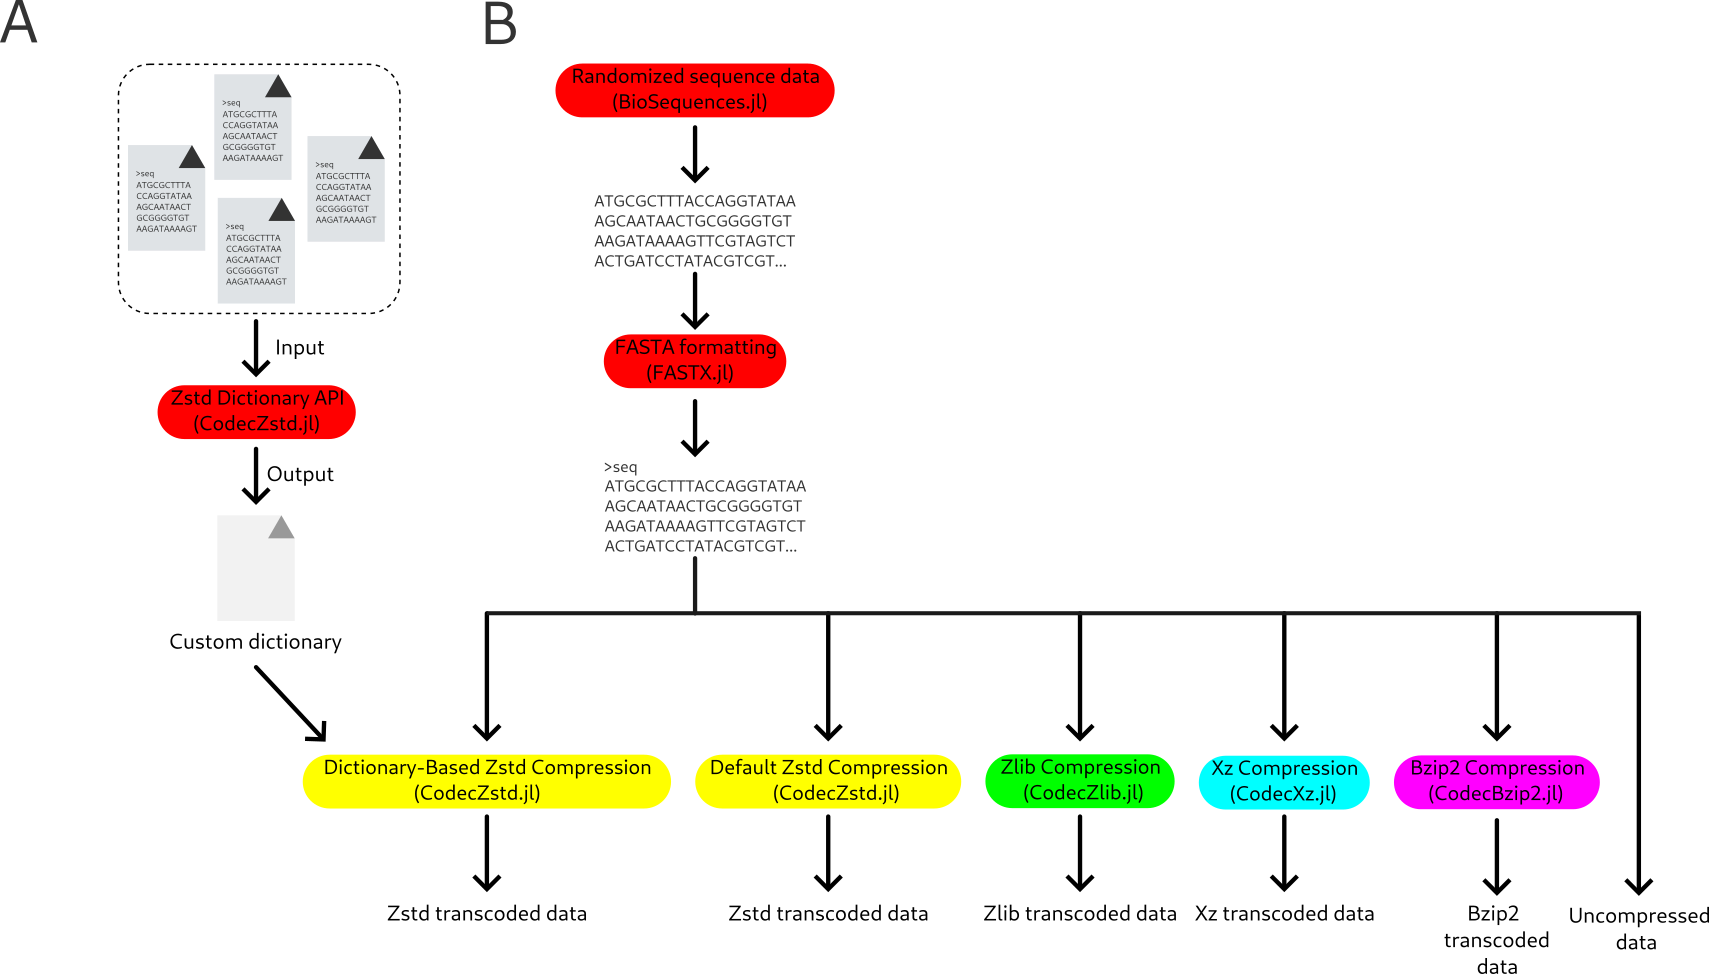
\includegraphics{/var/home/mpersico/distrobox/ubuntu-zstd/Persico2022/assets/figures/Compression_Pipeline_Model.png}

}

\caption{\label{fig-model}Overview of the Julia implementation for the
compression model. \textbf{A}, Custom dictionary generation via an Julia
artifact of FASTA files plugged into the Zstd Dictionary API.
\textbf{B}, Transcoding randomly generated FASTA formatted data using
TranscodingStreams.jl\citep{sato} compression codecs.}

\end{figure}

\hypertarget{results}{%
\section{Results}\label{results}}

\hypertarget{discussion}{%
\section{Discussion}\label{discussion}}

The provided FASTA training dataset was retrieved from a set of
\textit{E.coli} MS 200-1 strain genomic scaffolds from a whole genome
shotgun run\citep{ncbi}. Sampling a single organism may allow for
additional compression/decompression improvements as the sequence data
could possess repeating patterns unique to that individual's or species'
genome that are recognized and added to the Zstd dictionary during
training. The FASTA files themselves may bear similarity with one
another in the same set, such as each file being of similar length.
Simultaneously, the Zstd dictionary may not achieve comparable
compression/decompression performance when attempted on more dissimilar
sequence data. Portability of Zstd dictionaries, in the sense of being
universally applicable across all sequence data, could be weighed
against generating dedicated dictionaries for specific datasets
depending on the storage requirements. Zstd parameters were kept
default, though they can be manually altered, including advanced
compression options like compression job size or selecting from 22
predefined compression levels\citep{facebook}.

Zstd's multifarious design warrants further research in how tuning the
implementation by altering available options (block size, compression
level,\ldots) that might influence compression performance. The
development of novel data toolsets have utilized Zstd in unique ways.
Aside from the Nucleotide Archival Format, FASTAFS was recently
introduced as a filesystem in userspace (FUSE) toolkit wherein FASTA
files are pooled into a virtualization abstraction layer that archives
the set of data synced with its metadata, generating a high-level
interface for accessing and storing FASTA data\citep{fastafs}. The
zstd-seekable compression library is an embedded component that keeps
the FASTAFS archive compressed for storage reduction purposes, and it
represents an alternative compressed data format that deviates from
Zstandard, albeit in a compatible manner, that allows for partial
decompression of subranges of data\citep{facebook}. This is achieved via
independently compressed/decompressed Zstd frames, which FASTAFS
exploits for fast random access to FASTA files by decompressing only
data of interest. Further areas of research for general lossless data
compression in the context of biological data could include exploring
other properties like compression/decompression speed performance,
meaning how fast data transcoding occurs, or piloting proof-of-concept
algorithms that attempt novel strategies.

\hypertarget{supporting-information}{%
\section{Supporting information}\label{supporting-information}}

\paragraph*{S1 Fig.}
\label{s1-fig}
{\textbf{Bold the title sentence.}} Add descriptive text after the title
of the item (optional).

\paragraph*{S2 Fig.}
\label{s2-fig}
{\textbf{Lorem ipsum.}} Maecenas convallis mauris sit amet sem ultrices
gravida. Etiam eget sapien nibh. Sed ac ipsum eget enim egestas
ullamcorper nec euismod ligula. Curabitur fringilla pulvinar lectus
consectetur pellentesque.

\paragraph*{S1 File.}
\label{s1-file}
{\textbf{Lorem ipsum.}}

\paragraph*{S1 Video.}
\label{s1-video}
{\textbf{Lorem ipsum.}} Maecenas convallis mauris sit amet sem ultrices
gravida. Etiam eget sapien nibh. Sed ac ipsum eget enim egestas
ullamcorper nec euismod ligula. Curabitur fringilla pulvinar lectus
consectetur pellentesque.

\paragraph*{S1 Appendix.}
\label{s1-appendix}
{\textbf{Lorem ipsum.}} Maecenas convallis mauris sit amet sem ultrices
gravida. Etiam eget sapien nibh. Sed ac ipsum eget enim egestas
ullamcorper nec euismod ligula. Curabitur fringilla pulvinar lectus
consectetur pellentesque.

\paragraph*{S1 Table.}
\label{s1-table}
{\textbf{Lorem ipsum.}} Maecenas convallis mauris sit amet sem ultrices
gravida. Etiam eget sapien nibh. Sed ac ipsum eget enim egestas
ullamcorper nec euismod ligula. Curabitur fringilla pulvinar lectus
consectetur pellentesque.

\hypertarget{acknowledgments}{%
\section{Acknowledgments}\label{acknowledgments}}

I would like to express my sincere gratitude to Professor David Walsh
for teaching the bioinformatics course; My friends and family that
supported me throughout my studies; The Julia community for their
support before and throughout the writing of this paper; Mark
Kittisopikul for developing the CodecZstd.jl
\#dictionary\_and\_parameters branch for Zstd dictionary functions; The
Quarto developers for producing the Quarto publishing
system\citep{Allaire_Quarto_2022} along with the PLOS template used for
this paper; Luca Di Maio and contributors to the Distrobox tool for the
ease of setting up the containerized development
environments\citep{maio}; Maximiliano Sandoval and contributors to the
Citations app for managing the paper's bibliography\citep{sandoval}, and
all other persons that had indirectly assisted through their programs
and research.

\hypertarget{conflict-of-interest}{%
\section{Conflict of interest}\label{conflict-of-interest}}

The author declares no conflict of interest.


\nolinenumbers
  \bibliography{bibliography.bib}

\end{document}
